% !TeX spellcheck = en_US
\documentclass[sigconf]{acmart}

\usepackage{booktabs} % For formal tables
\usepackage{graphicx}
\graphicspath{{./images/}}
\usepackage{float}
\usepackage{amssymb}
\usepackage{booktabs}

% Copyright
%\setcopyright{none}
\setcopyright{rightsretained}

%Conference
% \acmConference[WOODSTOCK'97]{ACM Woodstock conference}{July 1997}{El
%   Paso, Texas USA} 
% \acmYear{1997}
\copyrightyear{2017}


\newif\ifworkinprogress
\workinprogresstrue

\definecolor{mygray}{gray}{.4}
\definecolor{darkgreen}{rgb}{0, .3, 0}
\definecolor{greenblue}{rgb}{0, .4, .5}
\definecolor{brown}{rgb}{0.59, 0.29, 0.0}
\definecolor{orange}{rgb}{1, 0.55, 0}
\definecolor{magenta}{rgb}{1, 0, 1}

\ifworkinprogress
\newcommand{\ce}[1]{\textcolor{blue}{[Chris] #1}}
\newcommand{\ez}[1]{\textcolor{red}{[Eva] #1}}
\newcommand{\ms}[1]{\textcolor{orange}{[Markus] #1}}
\else
\newcommand{\ce}[1]{}
\newcommand{\ez}[1]{}
\fi



\begin{document}
\title{Personalized music search based on graph embedding}


\author{Christian Esswein}
\affiliation{%  
  \institution{Databases and Information Systems}
  \department{Department of Computer Science}
  \state{University of Innsbruck} 
}
\email{christian.esswein@student.uibk.ac.at}


% TODO: word2vec is no tool, I + deepwalk used implementation of gensim!

\begin{abstract}
	% While exploring new music, users are typically limited to recommender systems which are proposing items either based on their listening history or on content similarities. Combining both methods models a "query-based recommendation" which enables users to filter content based on their preferences.
	% The ecosystem of music can be represented as an heterogeneous graph using all available data like tracks, artists, genres, tags and users. Using graph embedding techniques a low-dimensional vector representation is learned and provides a simple method to calculate similarities. Search queries, either single terms or combinations of items in the music graph, can be encoded using the same vector space. Therefore, not only exact results are found, but also similar items.
	
	Due to the rise of music streaming platforms, huge collections of music are now available to users on various devices. Within these collections, users aim to find and explore songs based on certain criteria reflecting their current and context-specific preferences. Currently, users are limited to either using search facilities or relying on recommender systems that suggest suitable tracks or artists. Using search facilities requires the user to have some idea about the targeted music and to formulate a query that accurately describes this music, whereas recommender systems are traditionally geared towards long-term shifts of user preferences in contrast to ad-hoc and interactive preference elicitation. To bridge this gap, I propose geMsearch, an approach for personalized, explorative music search based on graph embedding techniques. As the ecosystem of a music collection can be represented as a heterogeneous graph containing nodes describing e.g., tracks, artists, genres or users, I employ graph embedding techniques to learn low-dimensional vector representations for all nodes within the graph. This allows for efficient approximate querying of the collection and, more importantly, for employing visualization strategies that allow the user to explore the music collection in a 3D-space. To evaluate the approach, the tracks of Spotify playlists are predicted based on the playlist title.
	
	% This work presents an approach to create a personalized music search with Spotify data where new users can connect with their existing accounts. The retrieved results are not only presented in a list but instead the learned vector representation is exploited to generate 3D representations. For evaluation the content of playlists are predicted based on their title.
\end{abstract}


\keywords{Recommender Systems, Graph Embedding, Personalization}

\maketitle

\section{Introduction}
In recent years, music streaming platforms have become a central means for listening to music as these allow users to access huge collections of music. This evolution has also influenced the way users search and explore music. For instance, the streaming platform Spotify currently serves 140 million active users and provides a collection of more than 30 million songs\footnote{\url{http://press.spotify.com/us/about}} (as of June 2017). Consequently, the primary objective for users has shifted from retrieving specific songs to finding and ultimately exploring songs that match certain criteria reflecting the user's current preferences and context~\cite{lee2016look,kamalzadeh2012survey}. 

Currently, two paradigms allow users to explore large music collections: search and recommender systems. Utilizing naive search approaches based on simple attribute matching requires the collection data to be fully annotated with metadata. When relying on keyword search facilities, the user is required to have some idea of his/her current preferences and has to be able to formulate a query that actually describes these preferences well. More advanced search facilities are based on content similarities of items (aka ``find similar artists or songs'') and are rarely personalized. Especially data sparsity and the lacking ability for comparing heterogeneous items (tracks, artists, albums, etc.) makes it hard for such systems to succeed. In contrast, recommender systems propose items that might be suitable for the user(based on some collaborative filtering approach or more complex models. While recommender systems do not require the user to be able to formulate his/her current preferences, the user also is not able to directly influence recommendations by stating e.g., a starting point for his/her explorative search for music matching his/her current preferences (except for feedback mechanisms like relevance feedback and explicit ratings that influence the user model in the long term).

Only very few approaches like, e.g., the one proposed by Chen et al.~\cite{Chen:2016:QMR:2959100.2959169} allow the user to specify his/her current needs and preferences in an abstract manner, where the returned results are jointly based on the query (the user's current information need) and the user's personal music preferences. However, there is still a substantial lack of systems which combine flexible search mechanisms with user interfaces that provide dynamic, exploration-driven visualization strategies for large collections of music. 

Therefore, I propose the geMsearch system to bridge this gap in explorative music search. In particular, I propose to use graph embedding techniques for computing latent representations of items contained in the graph, such as tracks, users, artists, genres or acoustic features of tracks. Using such graph embedding techniques~\cite{yan2007graph}, a low-dimensional latent vector representation is learned for every node. These firstly allow to create advanced search facilities as search queries can be encoded in the same vector space. As a result, not only exact results can be retrieved, but also similar items and hence, exploiting previously unknown similarities between heterogeneous items that can be utilized to retrieve diverse search results. Secondly, the obtained vector representations can be exploited for advanced visualization paradigms enabling explorative music search which is beyond traditional list-based aggregations of search results that only provide a one-dimensional view of the retrieved items. 

%A desired search engine needs to learn a coherent latent representation for each item with some initial metadata and knowledge about item relationships in the training phase. 

%This work presents a preliminary study and visualization prototype based on latent representations obtained by graph embedding techniques. In contrast to traditional list-based aggregations of search results that provide a one-dimensional view of the retrieved items, we exploit the low-dimensional vector representation to generate 3D representations of the suggested items, allowing users to visually explore the music collection in a 3D-space. %Combined with the graph representation, query suggestions are provided. 
% The user is able to specify a starting point for his/her exploration of the musical 3D-space by browsing through this space, the query is implicitly refined and the user is provided with further suitable tracks and artists. 

\ce{describe model extensions}

% This work presents an approach to embed a Spotify dataset into latent representations to enable recommendations based on queries. 

The evaluation is performed on spotify dataset containing 852,293 tracks tracks. predict playlist tracks.
\ce{describe evaluation}

%After providing the first search results, the user should be assisted while exploring the remaining items and in the refinement of his search terms. Traditional list based aggregations of search results can only model a one dimensional view for the items. Instead of a list, the low-dimensional vector representation should be exploited to generate 3D representations of the suggested items. Combined with the graph representation, query suggestions can be provided.




\ce{adapt to this structure}
The remainder of this paper is structured as follows. In Section~\ref{sec:relwork}, we describe related work. Section~\ref{sec:viz_approach} proposes a visualization for explorative music search based on graph embeddings and presents the proposed prototype. We conclude the paper in Section~\ref{sec:conclusion} by summing up key aspects and detailing future work.

\section{Related work and background}

In this section related work is described from two fields: query-based recommender systems and approaches which focus on user interfaces for the exploration of new music. 

Recently, graph embedding techniques have also been introduced to the field of music information retrieval. Chen et al.~\cite{Chen:2016:QMR:2959100.2959169} utilize graph embeddings for realizing a query-based music recommender approach that is similar to the one presented in this paper. The main difference is that the music graph was modeled by Chen as a bipartite graph with users in one and all other items in the other set. This allows to create next track recommendations based on recent seed tracks. But item similarities are only constructed through collaborative filtering without content relationships because music items themselves are not connected in the initial graph. 

Chung et al.~\cite{chungexploiting} utilize a pure text-based music retrieval with the same dataset to predict the content of playlists with their title. A common latent representation of words and songs is learned with unsupervised learning based on their co-occurrence in playlist tracks and titles. However, only songs can be retrieved and the construction of queries is very limited. \\


For the task of building visualizations for music exploration, there are a number of relevant approaches, mostly based on proximity-preserving dimension reduction techniques. 

The Islands of Music interface~\cite{pampalk2001islands} incorporates rythm descriptors and employs self-organizing maps for visualizing music collections based on the metaphor of geographic maps in two-dimensional space. One highly relevant extension of these maps is a browsable 3D landscape by Knees et al.~\cite{knees2006innovative}, where tracks are clustered based on content features. %A similar approach uses inverse height maps for the computation of visualizations~\cite{lubbers2009adaptive}. 
Hamasaki and Goto~\cite{Hamasaki:2013:SMB:2491055.2491059} propose Songrium, a collection of visualization and exploration approaches. These include the ``Music Star Map'', a visualization of songs in a graph, where placement of songs is based on audio similarity. Also, Lamere et al.~\cite{lamere2007using} presented a 3D interface (Search Inside the Music) based on Multidimensional scaling techniques to visualize similarities between tracks, where each item is represented as a single colored item in the 3D space. Similarly, the Music Box visualization approach relies on Principal Component Analyses to visualize tracks, where song similarity is used to distribute tracks on a plane. %In contrast to the approach proposed in this paper, only tracks can be visualized, no clusters are used and album covers are involved in separate visualizations. 
The visualization proposed in this work differs from these approaches in the fact that I base the visualization on latent representations of items within a heterogeneous graph that includes tracks, artists, albums, genres, etc. Due to the applied graph embedding techniques, proximities within the graph visualization are not restricted to similarities between items of the same type (e.g., tracks) or similarities based on a single set of features (e.g., audio features), but rather capture the similarity of items of any type in the latent feature space.


\subsection{Background: Graph Embedding}
Graph embedding techniques aiming to transform graph structures into low a dimensional vector space. More formally, given a graph $ G = (V,E) $ with vertices $ V $ and edges $ E $ "a graph embedding is a mapping $ f : v_{i} \rightarrow y_{i} \in \mathbb{R}^{d} $ $ \forall i \in [n] $ such that $ d \ll |V| $ and the function $ f $ preserves some proximity measure defined on graph $ G $"~\cite{goyal2017graph}. The final result is therefore a vector representation of each node in the initial graph. Having this coherent search space makes it much easier to calculate higher-order proximities between heterogeneous nodes. Similar items can be retrieved using nearest-neighboring searches.

Existing embedding algorithms can in general be categorized into factorization based, random walk based and deep walking based methods. Concerning time complexity and preserved higher order proximities, mainly random walk based methods are interesting. Others methods either only embed similarities between connected nodes or their runtime is dependent on the number of edges in contrast to $ O(|V|) $~\cite{goyal2017graph}. The short random walks over edges are used to generate sentences which reflect the graph structure. Using this walks as training data, a representation for each word is learned. In the field of natural language processing this method is known as word embedding and especially popular with \emph{Word2vec}~\cite{mikolov2013efficient}. Both \emph{Deepwalk}~\cite{perozzi2014deepwalk} and \emph{node2vec}~\cite{grover2016node2vec} are making use of \emph{Word2vec} in their algorithms and reference implementations to embed arbitrary graph structures with random walks. For this work \emph{Deepwalk} was chosen because despite that \emph{node2vec} retrieves better embeddings in theory, it is not possible to extend the graph structure after its initial creation as explained in the section \ref{sec:model_extension}.

\section{geMsearch: Personalized music search}
In the following section, I present the geMsearch system, a first prototype for personalized explorative music search based on latent representations of nodes of the musical ecosystem\footnote{The prototype can be accessed at \url{http://dbis-graphembeddings.uibk.ac.at}}.
\emph{geMsearch} stands for graph embedding based music search and consists of two main components which are described in this and the following section: the graph embedding and retrieval engine that computes latent representations of items and query results, and the client providing a search and visualization interface. 


\subsection{Graph Embedding and Retrieval Engine}

% USE EXISTING TEXT

% whole process -> generate graph, embedd, compute

% graph, which data, why tags, users

% resulting embedding, properties, nearest neightbors are similar

% query example
% query construction: each item can be used, combining items, positive, negative, scaled user
% math notation

\begin{equation}
\tag{1}
q := 
\underbrace{
	\alpha_{x_{0}} * f(v_{x_{0}}) + ... + \alpha_{x_{n}} * f(v_{x_{n}})
}_{query \: intension} +
\underbrace{
	\alpha_{x_{u}} * f(v_{x_{u}})
}_{user \: preference}
\label{eqn:Stokes}
\end{equation}

% search refinement (as extra subsection?) -> each presented item can be used to extend query



% ----- graph -> embedding -----
For the creation of the graph underlying our approach, I rely on the Spotify playlist dataset by Pichl et al.~\cite{pichl2017improving}, containing 852,293 tracks crawled from public Spotify playlists. To enrich the available item descriptors for improved query performance, I also add Last.fm tags\footnote{\url{https://www.last.fm/api/show/track.getTags}} for the contained tracks. The resulting dataset is represented as a graph containing undirected edges between the following item types: user--track, track--tag, track--album, album--artist and artist--genre. For the computation of latent representations of nodes via graph embedding, I rely on the popular Deepwalk algorithm~\cite{perozzi2014deepwalk}, where I learn representations for all nodes in a 128 dimensional vector space. The resulting latent representations provides means for flexibly computing similarities between heterogeneous items such as tracks, users or artists. %and hence, retrieving exact matching items, but also similar items. 

% ----- query creation, user context, query eval -----
geMsearch allows users to interactively explore the music space to find new music. Therefore, a starting position for browsing through the items has to be determined by eliciting the user's current musical preferences. As can be seen in the top left corner of Figure~\ref{fig:web_client_query}, a text input field (with autocompletion support) allows to select multiple items from the dataset to construct a query that reflects the user's current preferences. Here, the search query for artist ``Jimi Hendrix'' may return similar and suitable artists, tracks or tags. In addition, the search result can further be restricted by adding further search terms. In Figure~\ref{fig:web_client_query}, the tag ``guitar'' is entered and combined with the first term. To create a search vector which is evaluated to retrieve nearest neighbors as search results, the mean item representation of these query terms is computed. The scaled user's latent representation is finally added to this vector and hence, long-term preferences partly influences the outcome. The resulting vector is then used to retrieve the most similar items from the graph as search results.
%In this combination each item could possibly be weighted to express either positive or negative short-term preferences. 

\iffalse
% ---------------- old part  ----------------
% TODO: use to adapt introduction?
	The increasing availability of huge music datasets through streaming platforms requires more sophisticated search methods to access desired tracks. Especially on streaming platforms, users expect to filter and consume music with predefined seeds like genres, context based scenarios or queries to find similar items of "x". This content based filters are in contrast to personal recommendations which are mainly based on historic listening behavior. To combine those two concepts and to allow users to specify arbitrary search intention, a flexible query system is required.
	
	The music corpus can be modeled in a heterogeneous graph with tracks, artists, album and tags as nodes and relationships as edges. Using graph embedding techniques as described in the previous section, a vector space with preserved proximities is created. Each item from the graph is included in the final embedding and can therefore be used as query term. Nearest neighbors represent similar items with decreasing proximity on higher distances. Because every query is formulated with vectors, also the combination of different search terms is possible. The retrieved items have mixed item types which means that not only tracks are returned but also artists for example. This is very powerful because neither user nor system have to decide at first hand the item type but can also easily apply filters. Another benefit is, that similarity measures between different item types are possible.
	
	the more graph structure is modelled, the better the resulting embedding gets. Including tags for tracks and genres for artists does solve two problems. On the one hand side, it models similarities between different items and therefore improves the embedding. On the other hand, it enriches the possible terms which can be used by users to construct queries. \\
	
	If user feedback is available, e.g. through historic track listening behavior or positive feedback on items, this data can be included into the graph. This improves the available graph structure and therefore may improve the embedding quality - collaborative filtering - and additional makes it possible to model a user preference on queries. For each user initiated search query, the user context is added and influences results with personal recommendations. Using the user without additional seed items even retrieves general recommendations with the same system.


	\subsection{Search refinement}
	
	% extend query
	Searching for music is not a single action process where a user formulates his information needs and then consumes the results. The search can be seen as a process where query refinements are always part of it. Therefore it is necessary that users are not only able to extend queries but also are supported with suggested terms. The user should feel like navigating through a virtual result space instead of jumping to unconnected places after manually modifying requirements. Having a search query which is represented as a vector, it can partially constructed as a combination of multiple search term vectors. This means that any of the proposed items can be used to further extend the query and refine the search.
	
	For example suppose that you first search for a music genre you are interested in and then find an artists in the results which matches your search intention. Adding this artist to the current query will not limit new results to the added artists but will return items which are similar to the genre and artist. Using this technique the user has not actively adapt the query through reformulating it and still gets more precisely results. \\
% / ---------------- old part  ----------------
\fi



\subsection{Model extension}
\label{sec:model_extension}

To alleviate the cold start problem for user profiles, users can connect to emph{geMsearch} with their Spotify account. The official Spotify API supports the OAuth protocol with different scopes, allowing access to, e.g., personal playlists, playing history or saved tracks. To create a personal preference profile, \emph{geMsearch} retrieves the user's saved tracks as I argue that saved tracks may serve as a strong indicator for preference. %In contrast, utilizing playing histories may contain noise. 
After a user has connected with his/her account, the music library is loaded and compared with the current contents of the underlying graph. For tracks, artists, etc. that are not yet contained in the underlying graph, I gather the missing metadata from Spotify and user-curated tags describing these items from Last.fm. After the data is collected, the graph is extended with this new information. In a next step, latent representations have to be computed in case of new items or updated in case of items that are affected by the newly added information.

\ce{connect with previous paragaph}
In real world scenarios, the dataset is not fixed and during runtime, more data is collected which needs to be included into the model. New data can either consists of new edges, e.g. new listening events of users during the use of the system, but also of new vertices when tracks or users are added. Especially if initial data is available for new users, e.g. through connecting with other services, a fast method is desirable such that the system can be used right away. A naive approach could simply recreate the whole embedding from scratch, but this is not scalable for bigger sets.



% Deepwalk uses short random walks to model the graph structure with an uniform distribution over nodes. Therefore, neither the complete graph structure, nor all nodes have to be known to the algorithm initially. This implies that additional nodes and edges can be added on-the-fly to continue learning and extending existing embeddings without the need to relearn the complete model from scratch when adding new users or items.
 

Random walk based embedding techniques are mostly online algorithms~\cite{perozzi2014deepwalk}\cite{grover2016node2vec} which can consume new walks during training as they are produced. This property is very powerful in general because for huge datasets not all walks have to be generated in advanced or even kept in memory. However, the probability distribution of random walks in \emph{node2vec} is not uniform and precomputed before walk generation based on the graph structure. This implies that neither edges nor vertices can be added or removed after the initial computation because it would invalidate previous transition probabilities.

On the contrary, \emph{DeepWalk} uses a uniform distribution over random walks and therefore allows graph structure extensions in theory. The presented algorithm and reference implementation does not offer this functionality but uses \emph{Word2vec} of Gensim~\cite{rehurek_lrec} to compute the actual embedding. Using \emph{Word2vec} in the backend makes it possible to store the current internal skip-gram model, later restore it for further learning with new sentences (walks) and additionally allows to extend the current vocabulary (vertices) during runtime. Combined the desired options are available to partially extend the existing graph and retrieve new embeddings.

\ce{check following paragraph}
To extend an existing embedding, first, new vertices and edges have to be collected and appended to the existing graph. Then new random walks are generated, but only over added vertices and edges. This new training data has only a small size compared to the initial data set and is proportional to the number of added structure. Then finally the existing \emph{Word2vec} model can be loaded, extended with new nodes, and learning is continued with new walks. \\


% Scalability:
With this method, graph and embedding can be updated with much less effort than relearning the complete model. However, even small changes can influence the whole embedding and create a new vector space. The scalability is therefore questionable because for big datasets the new embedding has to be updated completely which may invalidate all created indexes. Furthermore only graph structure can be extended but not modified or removed.

% TxODO: check percentage when adding node...
% TxODO: compare time between initial learning and extending: 3mins extending, 30min full model


\begin{figure}[ht]
	{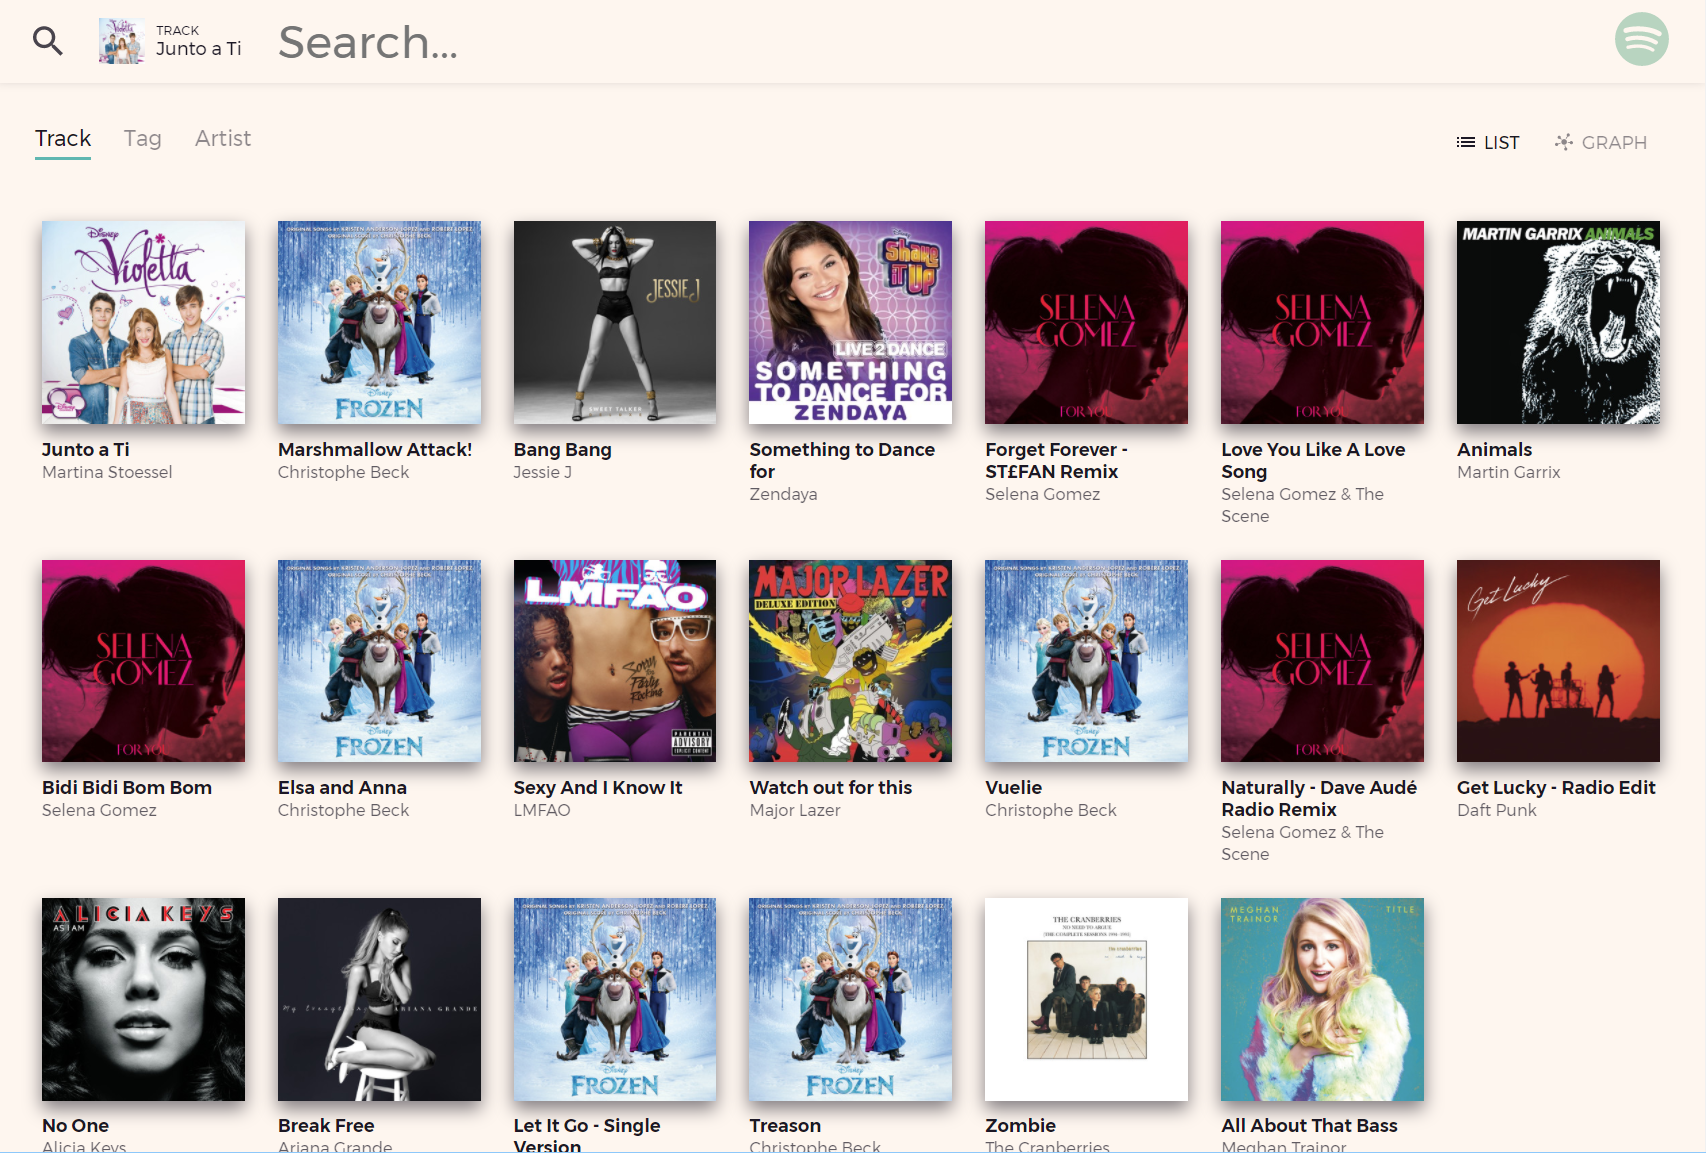
\includegraphics[width=250px]{web_client.png}}	
	\caption{Web client list results}
	\label{fig:web_client}
\end{figure}

\section{Visualization}
The most common visualization for both recommendation and search results is to display a list of items ordered by the predicted relevance of the individual items for the user. This limits users to only observing the sequential order of items and hence, a one-dimensional view agnostic to distances between consecutive items. With a latent feature space underlying the system (obtained through, e.g., graph embedding techniques), similarities between arbitrary items can be expressed which permits developing more advanced interfaces. Through recent advances in browser technology, like the availability of native WebGl, just-in-time visualizations of 3D scenes can be created directly on websites without complex precomputations or add-ons. 
%Also, users are nowadays more familiar with interactive and multidimensional interfaces. Enhanced result views could therefore may replace simple lists.
Using dimension reduction methods, the computed high-dimensional latent representations can be reduced to three dimensions, allowing to directly visualize items while preserving proximity. Here, I utilize principal component analysis to reduce the 128 dimensional representation of items to a three dimensional space. Instead of displaying a list of items, the recommended items can now be visualized in a 3D scene. Each track, artist or album can be positioned using its three-dimensional representation and can hence be displayed as an interactive 3D object. The positions and resulting distances reflect the relationships and proximities between items within the music collection. Beside the traditional list view for search results, the gemSearch client visualizes the surrounding items in a 3D WebGl scene as depicted in Figure~\ref{fig:web_client_3d}. Using such an interface does not only allow to express distance between items, but, more importantly, it allows the user to explore and browse through the result space interactively. Mouse gestures allow for exploring the virtual space and while navigating, additional items are lazy-loaded into the scene. 

% ----- search refinement, active + implicit -----
The user may first use a keyword search to express his/her current preferences (cf. section on Graph Embedding and Retrieval Engine). Based on these criteria, the first search results are retrieved and displayed in a 3D space, where the user should feel like navigating through a virtual result space instead of jumping to unconnected items. In the underlying latent vector space, any of the proposed items can be used to further extend the query and hence, refine the search to match current preferences more precisely. Besides this active manipulation, the 3D scene provides an even more effective process of implicit refinement. The most relevant search results are positioned around the center of the screen. When exploring additional items further away, the user has to opt for a direction in which to continue exploring. After inspecting items at the new position, the navigation direction can be refined. If the user detects suitable items, the direction is correct; otherwise the user will navigate in a different direction. This choice of directions and moving within the virtual result space directly translates to (implicit) query refinement. 


% ----- item representation and cluster -----
It is crucial to simplify the inspection of single items such that huge collections of music are explorable in reasonable time. I use album covers as textures for 3D objects describing track and album items and hence, also allow for visually inspecting node textures as this has shown to be an efficient means for judging the relevance of albums and tracks~\cite{libeks2011you}. To provide detailed information about selected items (e.g., artists of a given track, genres, etc.), information from the underlying graph is retrieved and displayed. Also, I provide music samples for each track that allow users to inspect and immediately consume newly discovered tracks. \\

As similar items are located in close proximity to one another in the resulting space, distance-based clustering techniques can be applied to represented accumulations of items as annotated clusters. This allows users to decide whether a set of items might be of interest by looking at the characteristics of the cluster and not having to inspect the individual items contained in the cluster. However, zooming in into a cluster to inspect the individual contained items is still possible. Figure~\ref{fig:web_client_3d} shows how clusters of similar items are represented as single orange circles. On click, the contained items are shown while all other elements are faded with transparency to enhance the contrast. As items within a cluster are positioned nearby, the scene  is zoomed in without scaling the circle sizes to avoid overlapping elements.


\begin{figure}[ht]
	{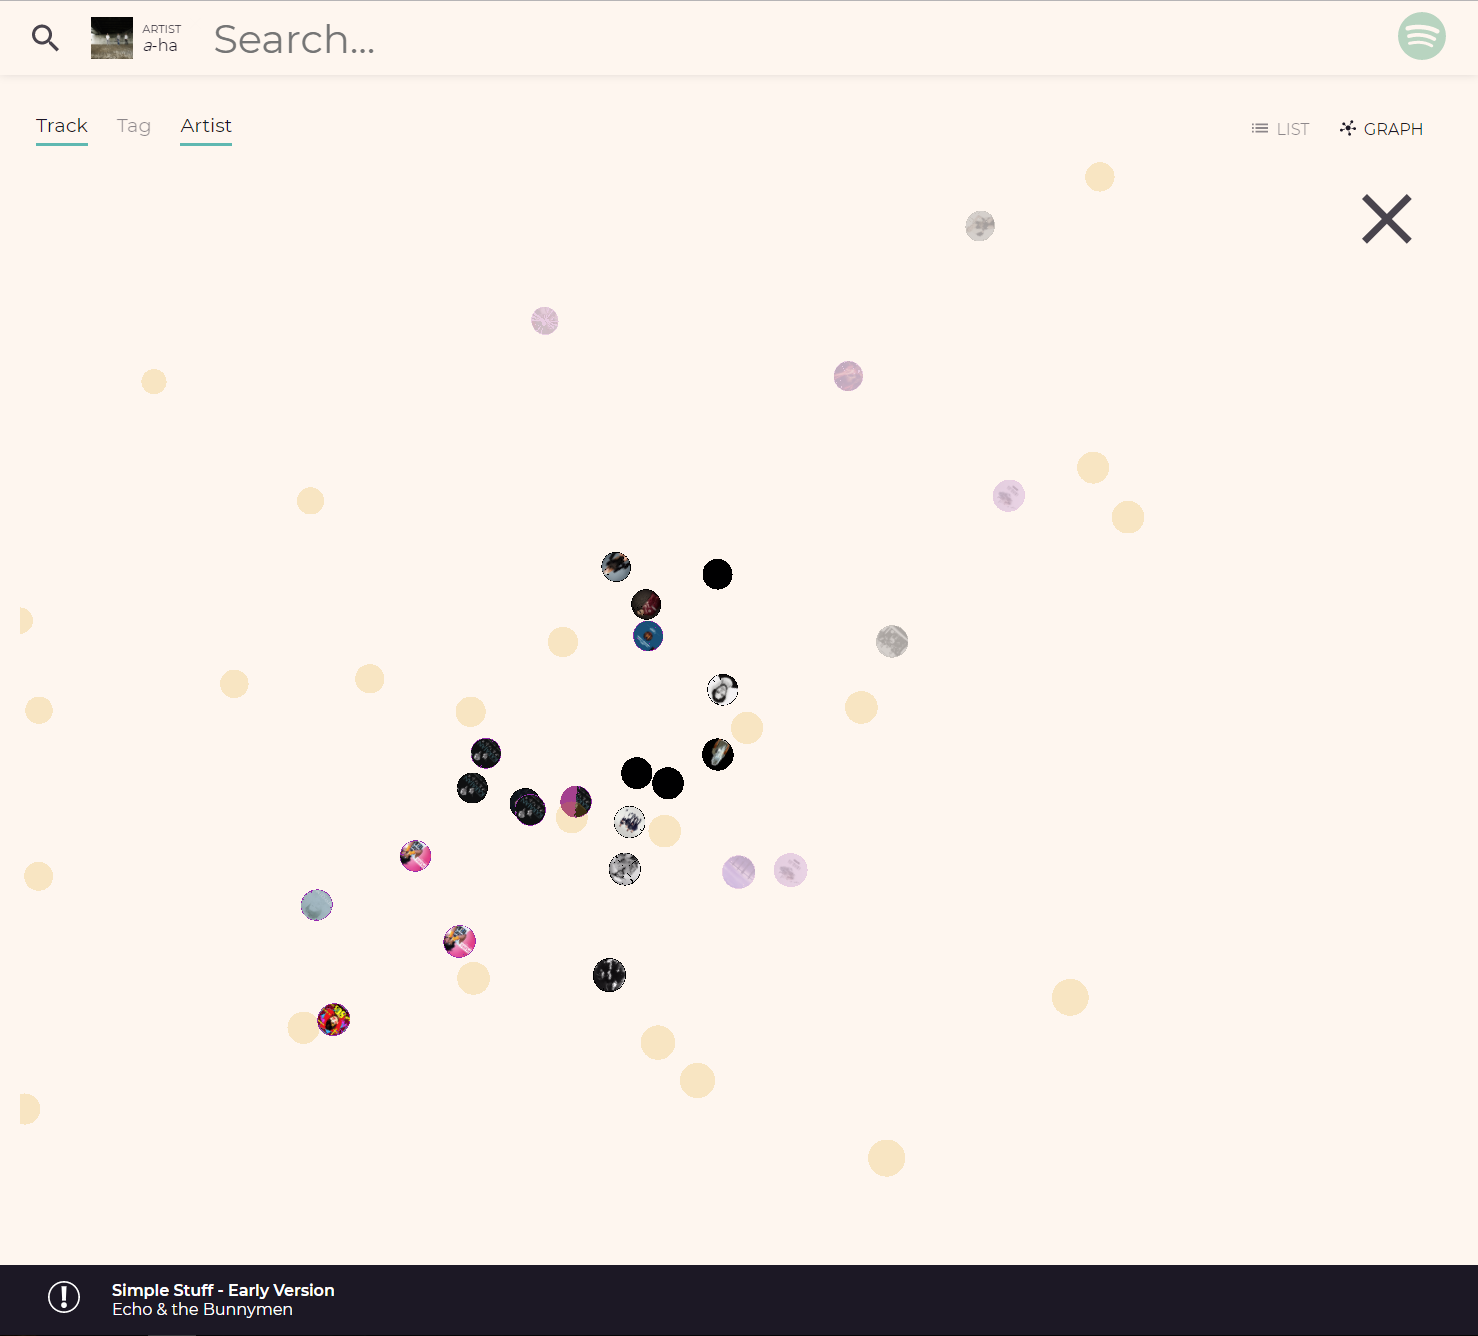
\includegraphics[width=250px]{web_client_3d.png}}	
	\caption{Web client 3D view and player bar}
	\label{fig:web_client_3d}
\end{figure}

\section{Experiments}
Estimating the quality of the presented approach is one of the key challenges because there exist no dataset which directly maps search queries with user context to results. Even having a working prototype client to test the system on real users, representative user studies require fairly big and diverse users bases. The test cases need to allow the users to estimate the results without being biased through available options or the test environment. A/B tests can model fair and solid results but require scopes in terms of number of users and participation which are only available on commercial platforms. Therefore, the common approach in research is to make use of crawled playlists which were manually created by users. As presented in \cite{kamehkhosh2017user}, this evaluations are comparable to user studies but require much less effort. Additionally, offline experiments can be easily repeated with adapted implementations and input parameters which helps during implementation and optimization to observe and benchmark the outcome. \\

Manually curated playlists can easily obtained, they have an user context and are usually labeled with a name. In a broader sense the contained tracks can therefore be seen as the desired output for queries by the name, related to the user. This is why the \emph{playlist evaluation}, further described in section \ref{subsec:playlist_eval}, uses the playlists as ground truth and tries to predict the tracks based on user context and playlist name. To evaluate the embedding quality in respect to personal preferences the \emph{track recommendation evaluation} in section \ref{subsec:track_rec_eval} compares user track recommendations to baseline methods.


\subsection{Dataset and graph generation}
The initial dataset was constructed from a crawled Spotify playlists by DBIS at the University of Innsbruck~\cite{pichl2017improving}. This data consists of playlists with an user context and contained tracks with artist and audio features. In order to enrich the available query terms and gather more graph structure, social curated track tags were crawled from \emph{Last.fm} \footnote{\url{https://www.last.fm/api/show/track.getTags}} and artist genres from Spotify.
%  \emph{Last.fm}\footnote{\url{www.last.fm}}

Because both the playlists and the \emph{Last.fm} tags where unfiltered user produced data, preprocessing was necessary. All playlists with less than four tracks or without an alphanumeric character in the title are removed. To match same tags on different tracks, the tag names are transformed to lowercase and special characters are removed. Tags with less than four characters, or without more than five user assignments on \emph{Last.fm} are also not included.

Table \ref{table:node_count} and \ref{table:edge_count} show which and how many elements and connections are contained in the graph after preprocessing. Within the dataset 12 tracks are most common for playlists.

\begin{table}[H]
	\caption{Node count by type:}
	\label{table:node_count}
	\begin{tabular}{lr}
		\midrule 
		\textbf{Type} & \textbf{Count} \\ 
		\midrule 
		Playlists & 21,336  \\
		Users     & 1,180     \\
		Tracks    & 852,293 \\
		Artists   & 110,377  \\
		Tags      & 395,587    \\
		Albums    & 189,174    \\
		Genres	  & 1,520	\\
		\midrule 
		Total nodes & 1,571,467\\
		\bottomrule
	\end{tabular}
\end{table}

\begin{table}[H]
	\caption{Edge count by types (undirected):}
	\label{table:edge_count}
	\begin{tabular}{lr}
		\midrule 
		\textbf{Type} & \textbf{Count} \\ 
		\midrule 
		Playlist-User   & 21,323  \\
		User-Tracks     & 1,662,605     \\
		Track-Album		& 852,293 \\
		Track-Artists   & 1,027,918 \\
		Track-Tags   	& 9,341,603 \\
		Artist-Genre	& 148,705  \\
		\midrule 
		Total edges 	& 13,054,447\\
		\bottomrule
	\end{tabular}
\end{table}

\subsection{Playlist evaluation}
\label{subsec:playlist_eval}
To predict playlist tracks based on the playlist title, two steps are required. First a query must be constructed from the title and then this query can be used to retrieve recommendations. Before running the evaluation, the total set of playlists is split into a training and a test set. Each user-playlist relation in the training set is used to create user-track edges in the graph which models the user preferences. With all available metadata the graph is completed and then embedded using Deepwalk. In the evaluation phase, for each playlist the title together with the user context is used to predict tracks which are matched against the actual playlist tracks. For the query extraction, terms in the title must be matched against known item names. To do so, the full-text search capabilities of \emph{Elasticsearch}\footnote{\url{www.elastic.co/products/elasticsearch}} are used. In the training phase all graph nodes except users and playlists are inserted into the database and are then available by their title as query terms. Having the high-level full text search, fuzzy matching and proximity queries are helping to match noisy items. Different techniques to extract and then combine multiple items to the final search vector are used which are discussed in the discussion section.

% TODO: different extraction techniques --> The first n retrieved items are used which results in better results through query expansion

To evaluate the performance, information retrieval measurements precision@k and recall@k are used. For baseline comparison a random track recommender returns random items for each playlist.

% TODO: also performance precisionOnHit


\subsection{Track recommendation evaluation}
\label{subsec:track_rec_eval}
In the presented model, queries are constructed using seeding elements combined with user context. Without seeds, the user alone can be used to query for recommendations. To perform a classic evaluation on user track recommendations, the playlists were used to construct historic track listening data, which is split into a training and test set per user. Using the training data, a new graph is generated and embedded. Then the users of the test set are used as queries to retrieve nearest neighbors in the embedding and compared with the test tracks. To measure the performance precision@10 and recall@10 are computed and compared against three baseline scores using \emph{MyMediaLite}~\cite{Gantner2011MyMediaLite}. Without personal context, the \emph{Random} method returns random items and the \emph{MostPopular} predicts tracks with the most overall listening counts. Whereas \emph{UserKNN} uses user-based collaborative filtering to predict k-nearest neighbors tracks. 


\section{Results and discussion}

As it can be seen in table \ref{table:track_rec_results}, the embedding can be used to produce personalized track recommendations which perform better than non-personalized methods and are nearly as good as standard matrix factorization techniques. Because this test data was constructed with the playlists, it confirms that playlists tracks can be seen in a user context.

\begin{table}[H]
	\caption{Track recommendation results:}
	\label{table:track_rec_results}
	\begin{tabular}{lrr}
		\midrule 
		\textbf{Recommender} & \textbf{Precision@10} & \textbf{Recall@10} \\ 
		\midrule 
		UserKNN   & 0.10468 & 0.0201  \\
		geMsearch   &  0.09468 &  0.0090  \\ % TODO: check recall value
		MostPopular   & 0.01872 & 0.00175  \\
		Random   & 0.00017 & 0.00001  \\
		\bottomrule
	\end{tabular}
\end{table}

The results of the playlist recommender are listed in table \ref{table:playlist_rec_results}. Compared with the random track recommender, the performance does clearly outstand. Furthermore they are better than the track recommendations which are only based on user preferences without seeding items. The experiments can not benchmark the query extraction and item retrieval separately.  \\
% TODO: different query extraction performacne....

Analyzing playlists without hits makes it clear that many playlist names are noisy and do not describe the contained tracks which makes it hard to predict the content. Furthermore about 48\% of the playlists contain tracks only from one artist. A nearer inspection shows, that often playlists are used to store albums or best-of collections of artists. As a consequence pure text-based methods on the same dataset can produce better results~\cite{chungexploiting}. In contrast, the here presented approach \emph{geMsearch} is designed to discover new music. Therefore the retrieved list of tracks is composed by a diversity of artists. Even the search results for a given artist does not guarantee to contain songs of the same artist in the top results. To reflect this desired outcome in the test data, the playlists are split into two disjunctive sets based on whether they contain tracks from multiple artists or not.

For playlists with tracks from only one artist the overall performance is much better but the user as part of the query does not improve the results. 


Currently personalized recommendations can be created, but the effect in combination with queries is not as strong as expected. 
--> hard to explain whether the current approach to construct the search vector is not correct or if the evaluation with playlist data can not reflect the desired outcome.

\begin{table*}
	\caption{Playlist recommendation results:}
	\label{table:playlist_rec_results}
	\begin{tabular}{lrrrr}
		\midrule 
		\textbf{Recommender}& \textbf{Precision@1} & \textbf{Precision@10} & \textbf{Recall@10}& \textbf{PrecisiononHits@10} \\ 
		\midrule 
% TODO: insert results
		UserKNN   & 0.10468 & 0.0201  \\
		geMsearch   & 0.08827 & 0.003  \\
		MostPopular   & 0.01872 & 0.00175  \\
		Random   & 0.00017 & 0.00001  \\
		\bottomrule
	\end{tabular}
\end{table*}



As expected, more structural data provided through the graph creates better embedding and therefore more meaningful results. Especially tags assigned to tracks improved the precision scores for the playlist track prediction by XX\%. % TODO: integrate number


\section{Conclusion}
This work presented an approach to use graph embedding techniques to create a low dimensional vector space of music data. This embedding is used to create query-bases music recommendations and evaluated against playlist track predictions. Combined with a 3D representation of the result items it improves the way how user find and explorer new music. 
This method is not limited to music and may be also used in different domains where application data can be represented as graph but metadata for single items is sparse.

There is still potential for future work in order to improve the embedding itself and also the query mechanism.  Weighted graphs seemed to be a promising approach to improve the embedded proximities in early tests. It could also be possible to even include audio features as graph nodes in order to introduce audio similarities.


\bibliographystyle{ACM-Reference-Format}
\bibliography{bibtex}


\newpage
\appendix
\section{Implementation Details}

The implementation can be structured into two main components. As it can be seen in figure \ref{fig:architecture} the data management, graph embedding and recommendation computation is implemented as a Python application. With a REST interface this services are exposed and decoupled from the second component, the web client.

\begin{figure}[ht]
	{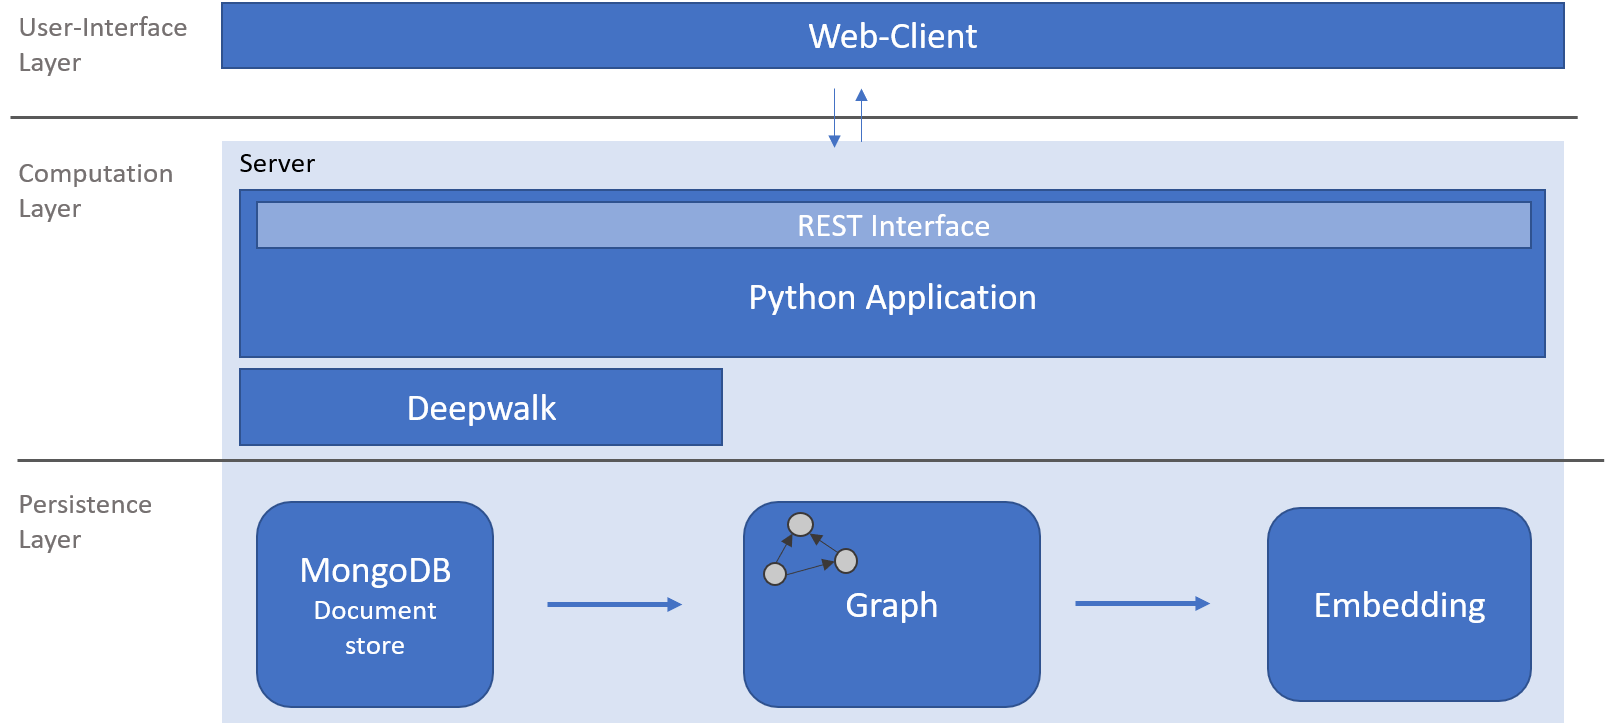
\includegraphics[width=250px]{architecture.png}}	
	\caption{Main architecture overview}
	\label{fig:architecture}
\end{figure}

\subsection{Python application}
The actual recommender is implemented in Python because many packages for data processing and machine learning exists. In addition also the reference implementation of \emph{Deepwalk} and the tool \emph{Word2vec} are written in Python. To achieve reasonable runtime performance, big data structures are stored and accessed with the Python package \emph{numpy} and matrix computations are performed with \emph{scipy} which both rely on native implementations.

% TODO: graph generation, embedding using deepwalk (a modification to enable model extensions)
% PCA for dimension reduction. Other methods where tested but where not fast enough on the big dataset.

\subsection{Data management}
The main data source for geMsearch is the Spotify API where DBIS has already crawled a big dataset~\cite{pichl2017improving}. Because this data is stored as JSON, the NoSQL document store \emph{MongoDb} is used to store all crawled data. This makes it easy to create data subsets for testing, performing statistic analyses and retrieving metadata to enrich the search results. Synchronized user music libraries are also stored here.
For embedding and evaluation required data is extracted and stored as CSV files in an intermediate step. This makes is easier to process or split data and repeat experiments with same sub-data inputs. After potential training-test splits are applied, the music graph is constructed. When adding new data to the graph a mapping for item ids is applied which makes sure that each node is identified by a unique integer id. This continuous ids are required for the graph embedding algorithms as input and later to transform an embedding index back to the original item. Additionally they make sure that same items, e.g. text equal tags, are represented as a single node in the graph. \\

Each item which has a name except playlists and users are inserted into a \emph{Elasticsearch} full-text index. For the evaluation based on playlists, this service is used to extract query terms from the playlist title. Also the client makes use of this index service to provide an autocomplete function for users while formulating queries.

\subsection{Webclient}
% TODO: copied from previous
\ce{merge / remove}
Supported with autocomplete suggestion the user can select any item of the graph to formulate single or combined queries. To provide recommendations, this selection is send to the API server instance and evaluated on the embedded graph. Filters can further restrict the search results for certain element types, like tracks, tags or artists. Before sending results to the client, additional metadata like artist names for tracks and album covers are queried from a simple document store and added to the response. Because of its popularity and easy to use API the data highly depends on the Spotify API. This ensures a high availability of metadata as well as album covers and makes it possible to play short sound samples for each track.\\



The implemented Webclient makes it possible for users to formulate queries and explorer recommendations. Without the need for an installation or additional setup, the web application has many advantages over traditional desktop applications. \emph{TypeScript}, a programming language superset of JavaScript, was chosen for the implementation because it provides static type checking during compilation. Created and maintained by Microsoft it also enables strong autocomplete suggestions in their editor \emph{VS Code} which improves the development process. \\
The JavaScript framework \emph{React} helps to maintain the client state and having a virtual DOM enables to program on a more abstract level as no direct DOM manipulations have to be applied. The whole client is a standalone application and communication with the Python API is done via REST interface to retrieve search results and metadata. Hereby both components are independent and additional or different clients could possibly be introduced. \\

Beside the list view, results can also be explored in a 3D scene where each item is represented as single interactive object. For performance reasons this scene is rendered in a canvas element using WebGL which is hardware accelerated on most devices. WebGL has currently many crossbrowser issues in different browsers and requires to write shader codes for simple visualizations. The JavaScript library \emph{ThreeJS} fixes this issues with a common API and simplifies the development with many utility methods.

For exploring the search results, users can modify the scene camera position using their mouse and navigate through the 3D space. The whole embedding is too big as it could be transfered complete to the client. Therefore only the most accurate results are returned for queries and additional items are loaded step by step. After each position change, the camera direction is unprojected to get the focused 3D position. Having the new center, additional elements can be queried and added to the existing scene.

\subsection{Spotify Connector}
As described in section \ref{sec:impl_spotify_connect}, a Spotify account can be used to get personalized recommendations. When a user connects, access to the username and the personal music library is granted. The OAuth protocols allows to retrieve this data as a third party application without knowing the users login credentials. Only a token is transmitted which authorizes API request for a limited time.

After the user has connected, it is checked if he is already known in the system. For new users, the token is send to the server in order to synchronize the music library. In the database this user data is only identified by the hash of the username and prevents backtracking of personal information.\\

Besides the API there are two microservices on the server which execute long running tasks and prevent to block resources for further requests:
\begin{itemize}
	\item The \textbf{Crawler service} watches the database for new tracks which are inserted through the music library synchronization. It makes sure that all necessary metadata is available. For new items, track and artists are crawled from Spotify and tags for tracks are retrieved from Last.fm.
	\item The \textbf{Embedder services} waits until crawlers are finished and then extends the existing graph with new the data. This task is executed periodically and therefore may embed multiple users at once. Changes are collected and then inserted into the existing Word2Vec model to retrieve a new embedding which then replaces the existing one.
\end{itemize}


\end{document}
